\documentclass[11pt]{article}
\usepackage{amsmath, amssymb, amsthm}
\usepackage{geometry}
\usepackage{graphicx}
\usepackage{hyperref}
\usepackage[backend=biber]{biblatex}
\addbibresource{../references.bib}
\geometry{margin=1in}
\title{Informational Equivalence and Entropy Collapse in Black Hole Simulation}
\author{Juha Meskanen}
\date{2024}

\begin{document}
\maketitle

\begin{abstract}
  Building on our earlier proposal that the universe is fundamentally informational in nature, we present a computational model of black hole singularities based on the entropy of execution traces. By simulating black hole evolution as a computational process, we represent system states as bitstrings and define a mapping from informational content to emergent spacetime geometry. We demonstrate that vanishing Shannon entropy corresponds to geometric collapse into a singular point across all embedding schemes. A Python simulationS illustrates this entropy--geometry correspondence based on various collapse scenarios. These results support the view that geometric singularities may emerge from informational degeneracy and suggest that entropy defines an absolute informational metric for geometry.
\end{abstract}

\section{Introduction}

This paper builds on a previously proposed framework in which physical reality, including time and conscious experience, emerges from the execution of formal axiomatic systems \cite{meskanen2019}. In that framework, both physical and simulated observers are regarded as equivalent configurations of information. We now extend this idea to spacetime structures, specifically black holes, and explore how geometric singularities manifest under an informational ontology.

This leads to the central theoretical claim of this paper:

\begin{quote}
  \textbf{Lemma (Entropy--Singularity Lemma):} \emph{Vanishing entropy implies geometric singularity.}
\end{quote}

We formalize this claim by simulating the evolution of a gravitationally collapsing system using discrete bitstring representations and analyzing the entropy of its execution trace.

\section{Methods}

We model black hole evolution as a computational process where spacetime states are encoded in quantized memory images. These are serialized into bitstrings that evolve over simulated time steps. The simulations need not reach the singularity to provide insight; instead, we extrapolate the entropy trend toward completion. These simulations are implemented in Python and publicly available at:

\url{http://githumb/juhakm/}

Due to computational challenges black hole is assumed static, and mass-energy accumulation or backreaction is not included.

Our goal is to understand the qualitative behavior of the informational representation of spacetime near singularity conditions.



\section{Execution Trace as Measure of Shannon Entropy}

Let $\mathcal{M}$ be the set of all memory locations. A machine state $s \subseteq \mathcal{M}$ includes the values of memory, registers, and CPU state.

Let $S$ denote the set of all possible machine states, and let a program be a finite sequence of instructions:
\[
  P = (I_1, I_2, \dots, I_n)
\]
Each instruction $I_i$ induces a transition $I_i : S \to S$.

The execution trace is the ordered sequence:
\[
  T = (s_0, s_1, \dots, s_n) \quad \text{where } s_{i+1} = I_{i+1}(s_i)
\]

The corresponding transition relation is:
\[
  R_P = \{ (s_i, s_{i+1}) \in S \times S \mid s_{i+1} = I_{i+1}(s_i) \}
\]


\subsection{Mapping Bitstrings to Geometry}

Let a complete system state be encoded as a bitstring $b \in \{0,1\}^L$. Each such bitstring is interpreted as a discrete geometric state.

Let:
\[
  \mathcal{C} = \{0,1\}^{3k}
\]
be the space of 3D geometric configurations. Define:
\[
  f : \mathcal{C} \to \mathbb{Z}^3, \quad f(b) = (\phi(b_1), \phi(b_2), \phi(b_3))
\]
where $\phi : \{0,1\}^k \to \mathbb{Z}$ decodes fixed-length binary segments into integers. This mapping allows us to represent evolving spacetime geometries as trajectories in discrete space.


\section{Entropy Collapse and Geometric Singularity}

We define the empirical Shannon entropy over the execution trace $T$ as:
\[
  H(T) = -\sum_{s \in T} p_T(s) \log_2 p_T(s)
\]
where $p_T(s)$ is the empirical frequency of state $s$ in $T$.

When $H(T) \to 0$, the system visits a single state repeatedly, implying no informational variability. Since all geometric mappings of such a state yield the same output, the corresponding spatial representation degenerates to a single point.

\begin{quote}
  \textbf{Entropy--Singularity Lemma (Formal Statement):} \\
  Let $T$ be an execution trace of bitstrings mapped via $f$ to $\mathbb{Z}^3$. Then as $H(T) \to 0$, the image $f(T)$ collapses to a singleton set. That is:
  \[
    H(T) \to 0 \quad \Rightarrow \quad \exists p \in \mathbb{Z}^3 \text{ such that } f(s_i) = p \text{ for all } s_i \in T
  \]
\end{quote}

\subsection*{Justification}

This lemma holds regardless of the specific geometric interpretation. Bitstrings with no entropy (i.e., constant or nearly constant) encode no distinguishing information. Therefore, any function $f$ that interprets structure from such data yields an invariant point in geometric space. This outcome is invariant under changes of representation, including dimensional projection, coordinate transformation, or encoding scheme.

\section{Simulation of Schwarzschild Collapse}

Three different models were studied:
\begin{itemize}
  \item schwarzchild\_entropy.py: Computationally light approximation
  \item schwarzchild\_geodesic.py: Geodesics solved to the singularity using Radau method.
  \item schwarzchild\_eddington\_finkelstein.py: Geodesics solved with Eddington-Finkelstein coordinates.
\end{itemize}

These simulate massless dust particles collapsing under a Schwarzschild geometry using a discretized geodesic model. Particle positions are serialized into bitstrings, from which entropy is computed. Integer encoding of coordinates was used to isolate physical entropy from artifacts of floating-point representation, ensuring that Shannon entropy reflects only the simulated spacetime's informational structure.


\begin{figure}[h!]
  \centering
  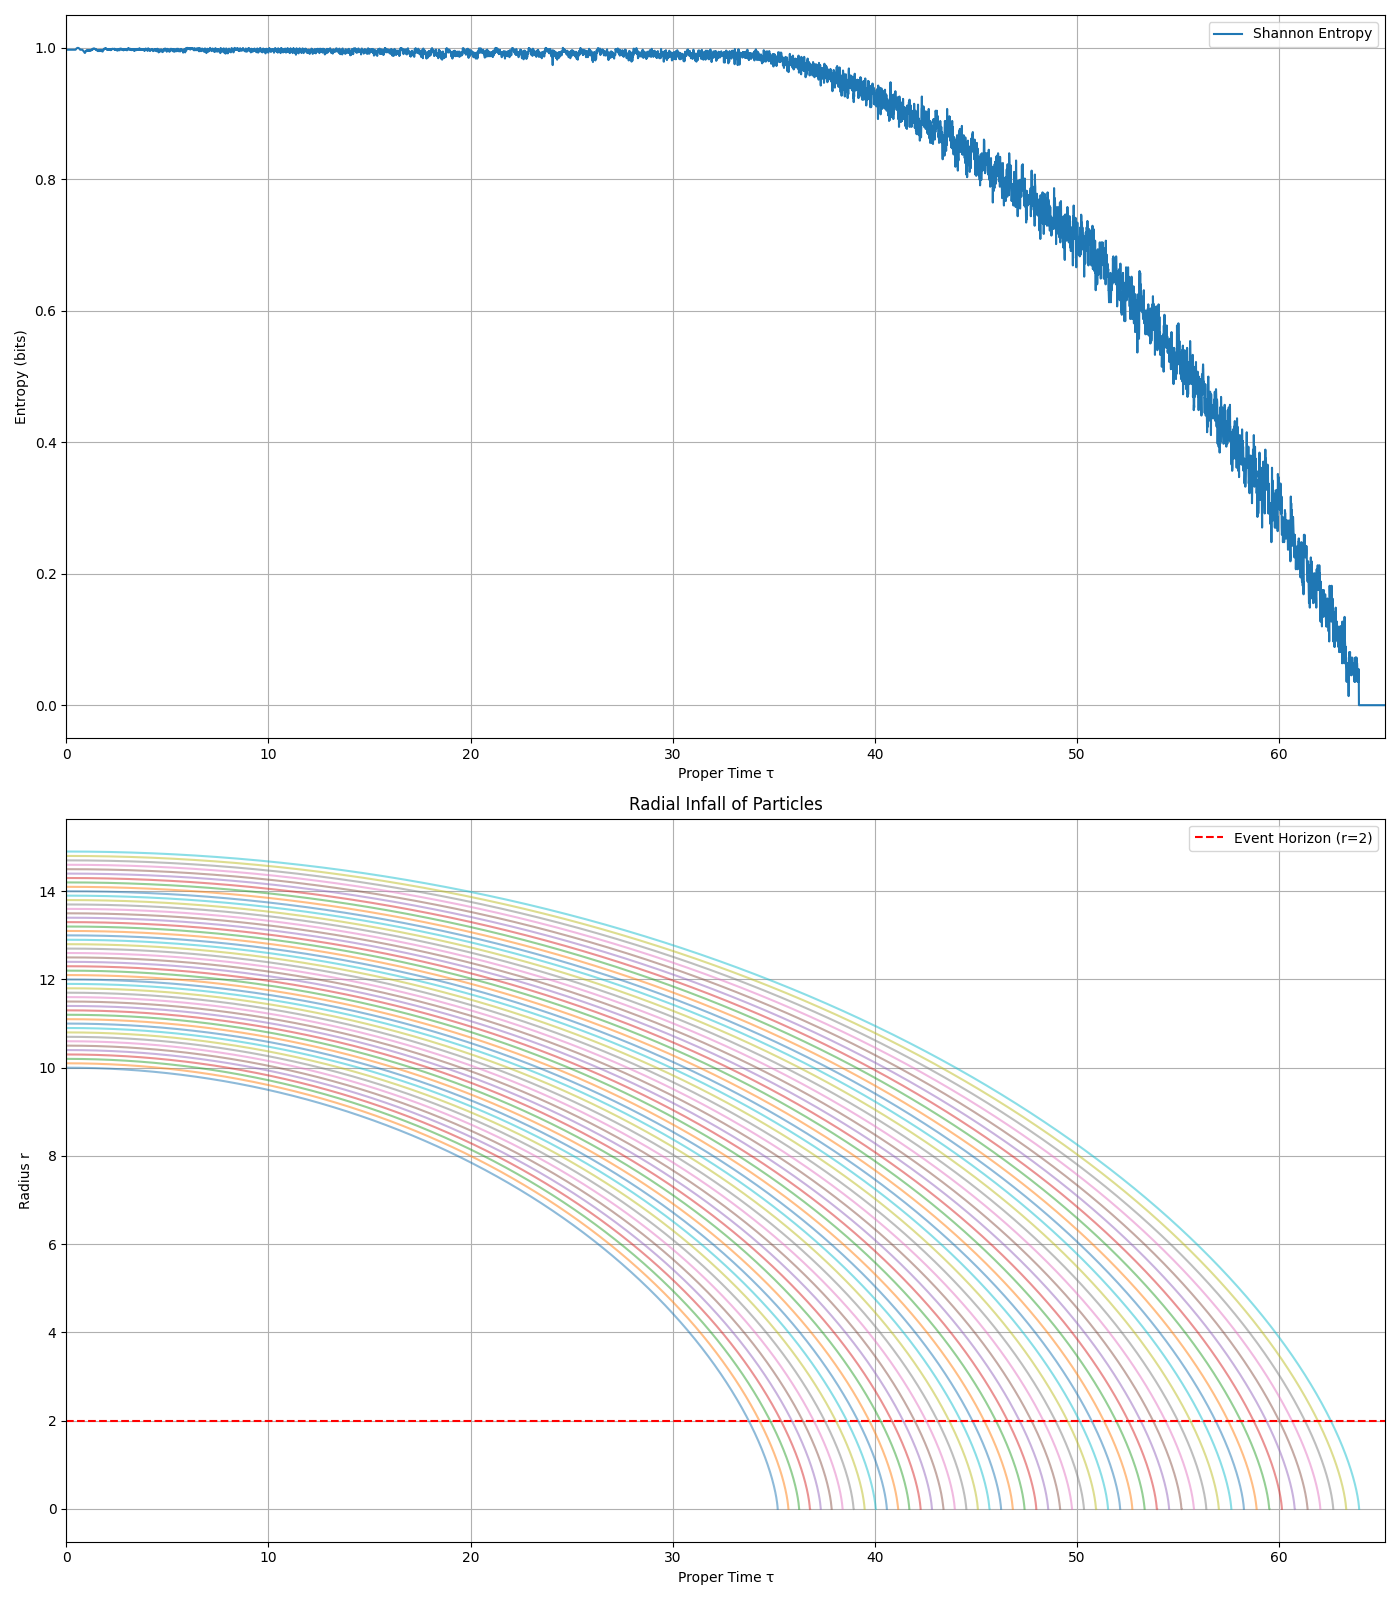
\includegraphics[width=\textwidth]{figures/schwarzschild_entropy_signature.png}
  \caption{Entropy signature during collapse. As particles approach the singularity, entropy of state bitstrings decreases, indicating reduced configurational freedom and increasing informational degeneracy.}
  \label{fig:schwarzschild_entropy}
\end{figure}

\begin{figure}[h!]
  \centering
  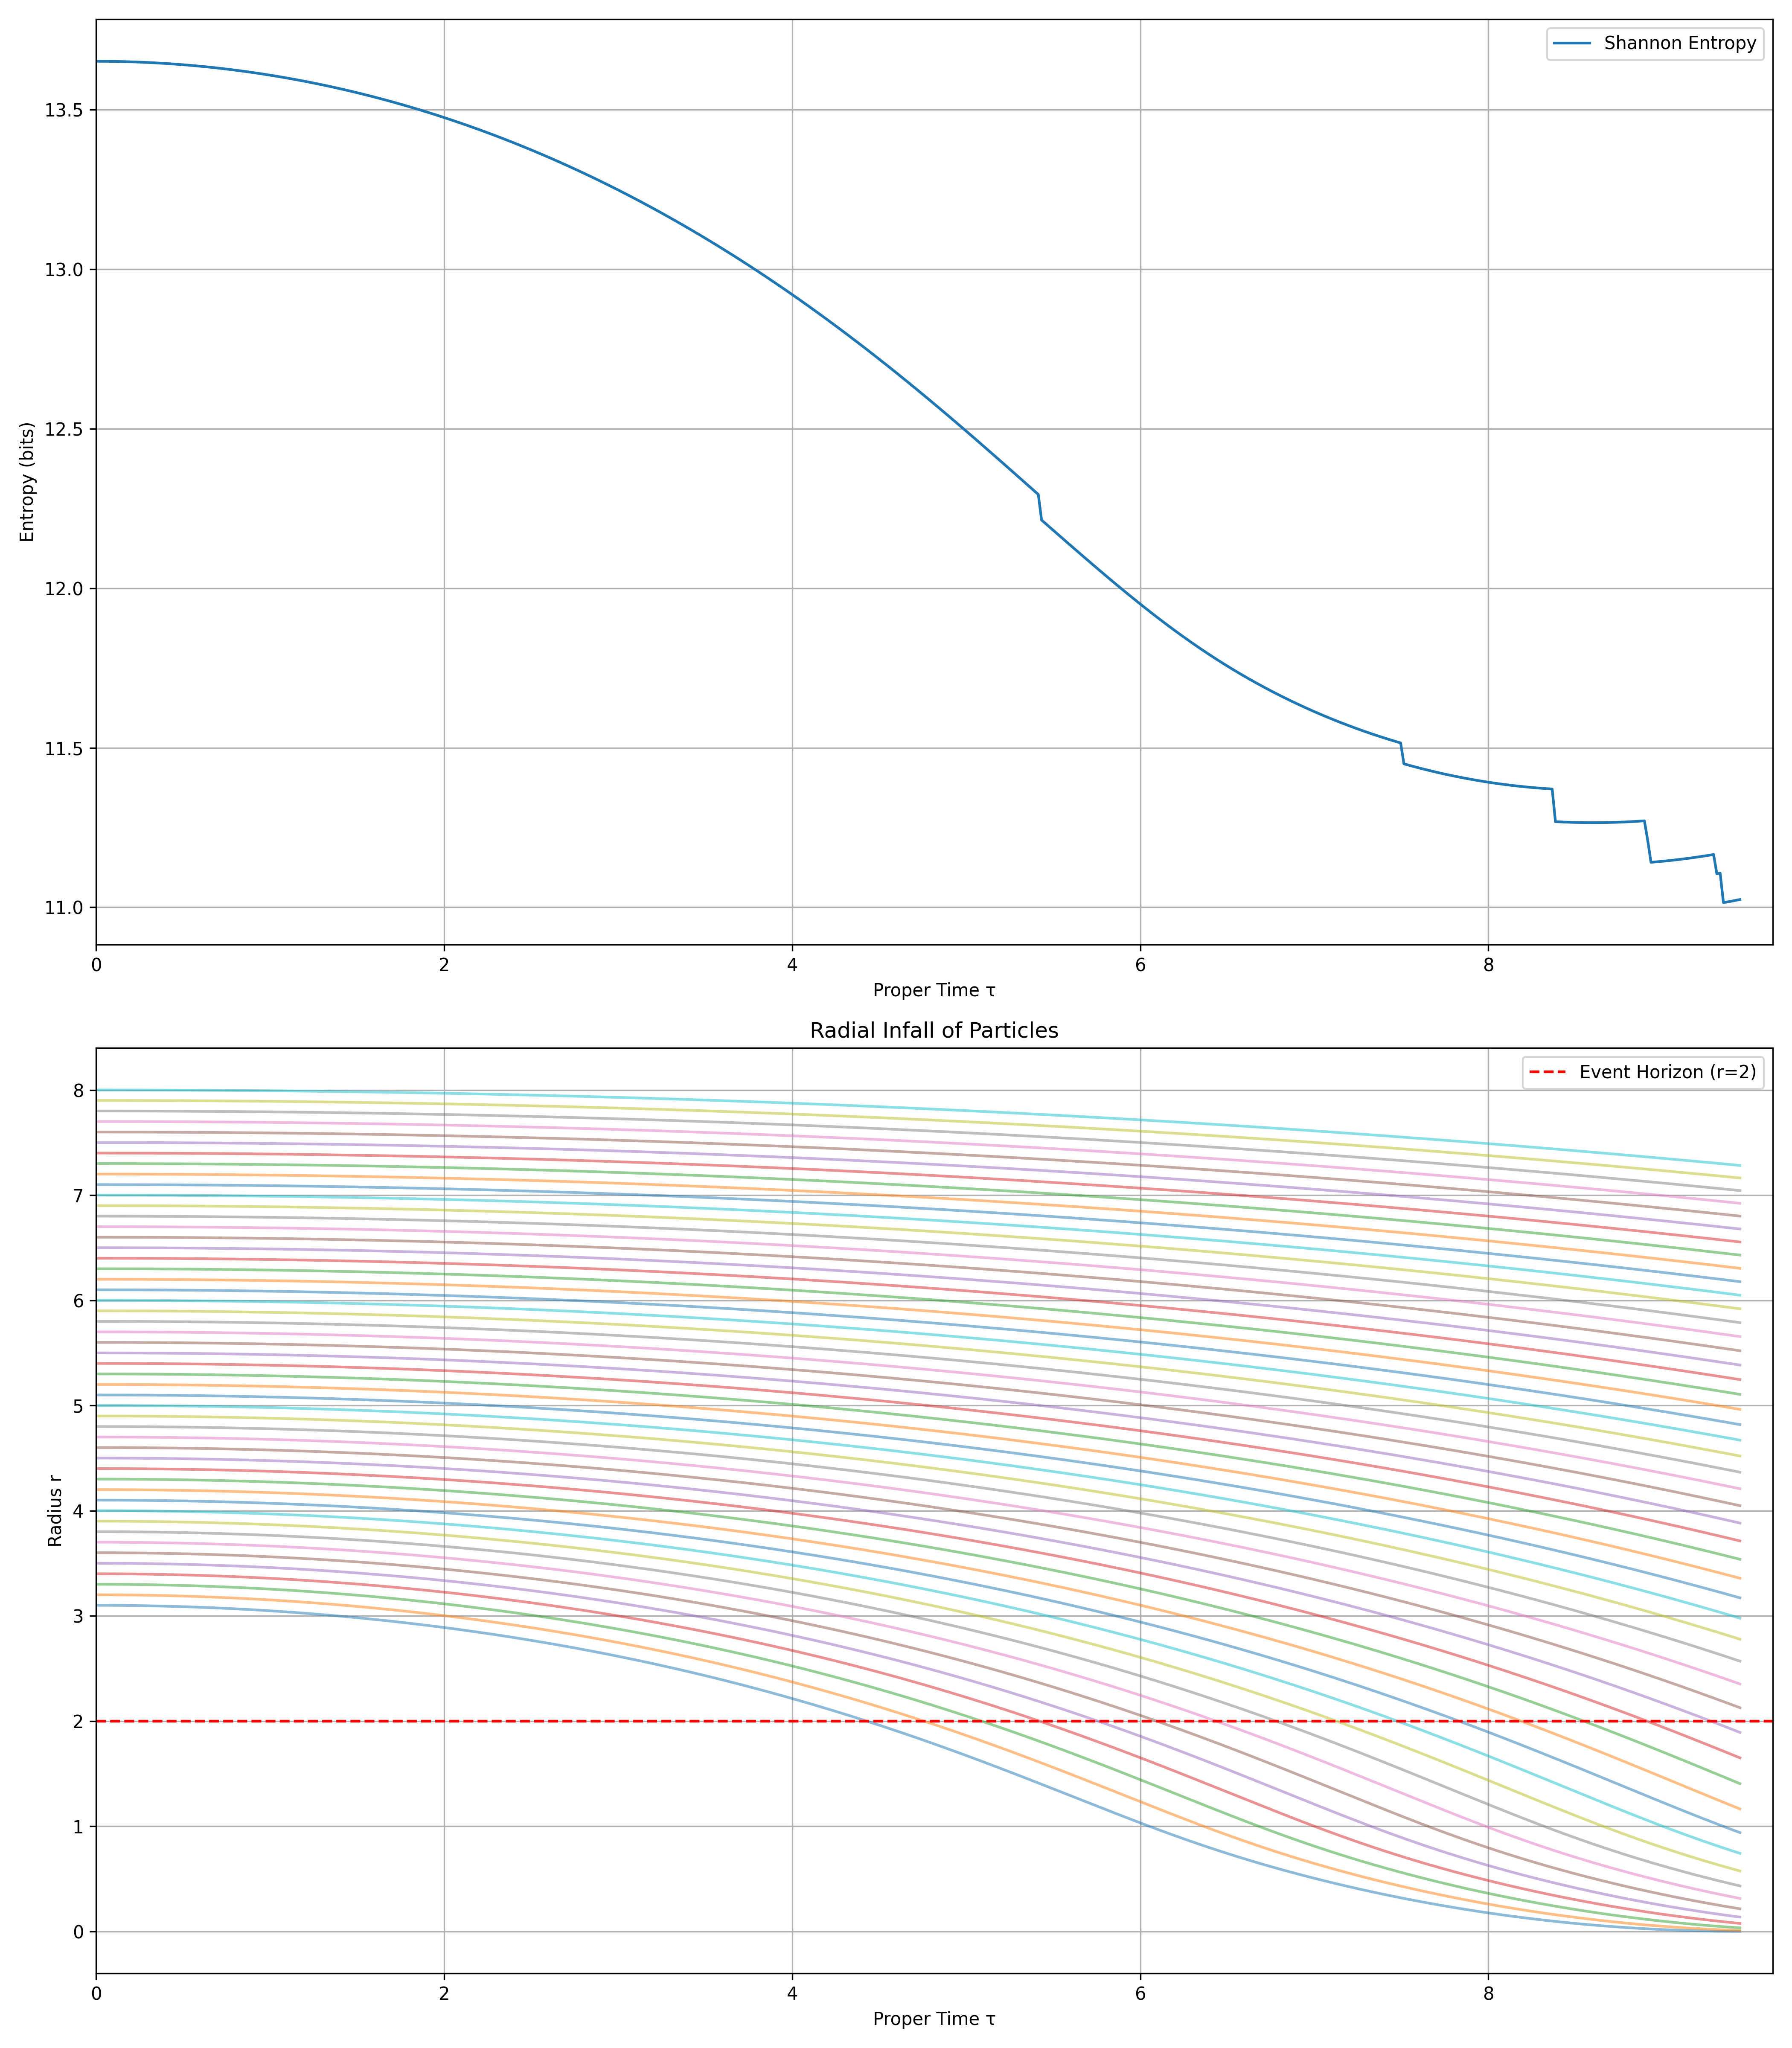
\includegraphics[width=\textwidth]{figures/schwarzschild_radau.png}
  \caption{Entropy signature of trajectories integreated with Radau method.}
  \label{fig:schwarzschild_radau}
\end{figure}

\begin{figure}[h!]
  \centering
  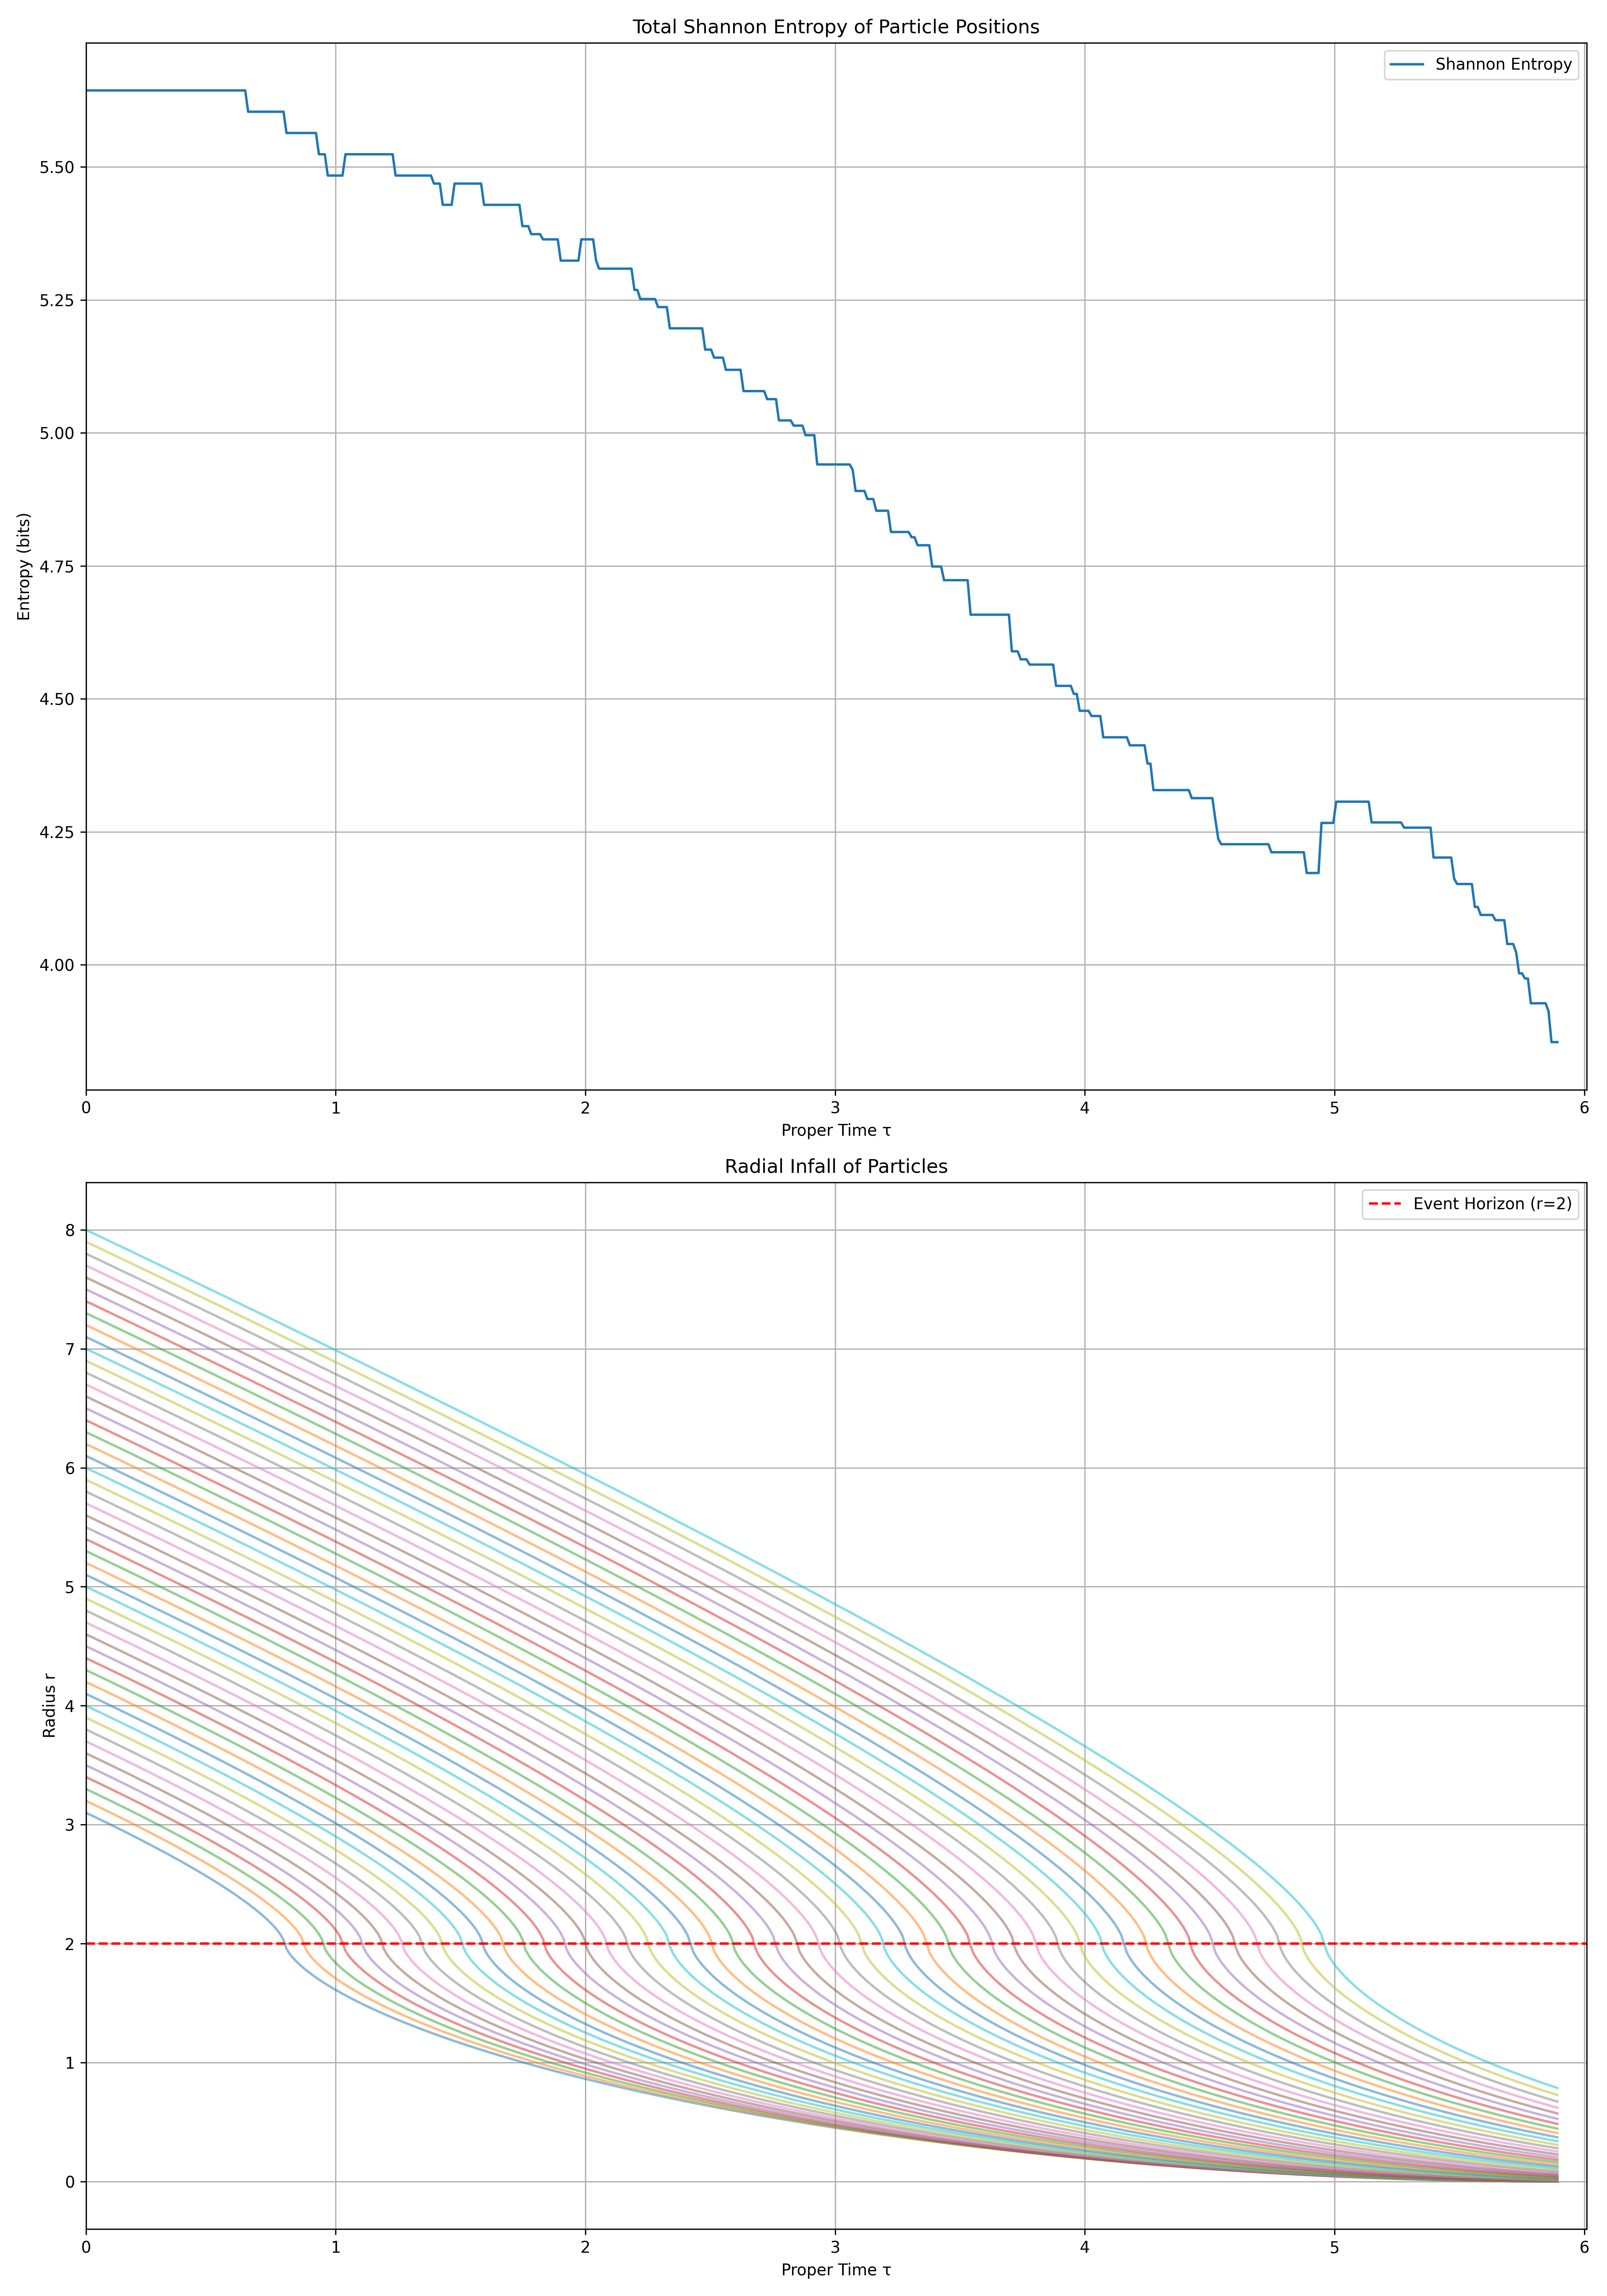
\includegraphics[width=\textwidth]{figures/schwarzschild_eddington_finkelstein.png}
  \caption{Entropy signature of trajectories integreated with Eddington-Finkestein coordinates.}
  \label{fig:schwarzschild_eddington_finkelstein}
\end{figure}


\begin{figure}[h!]
  \centering
  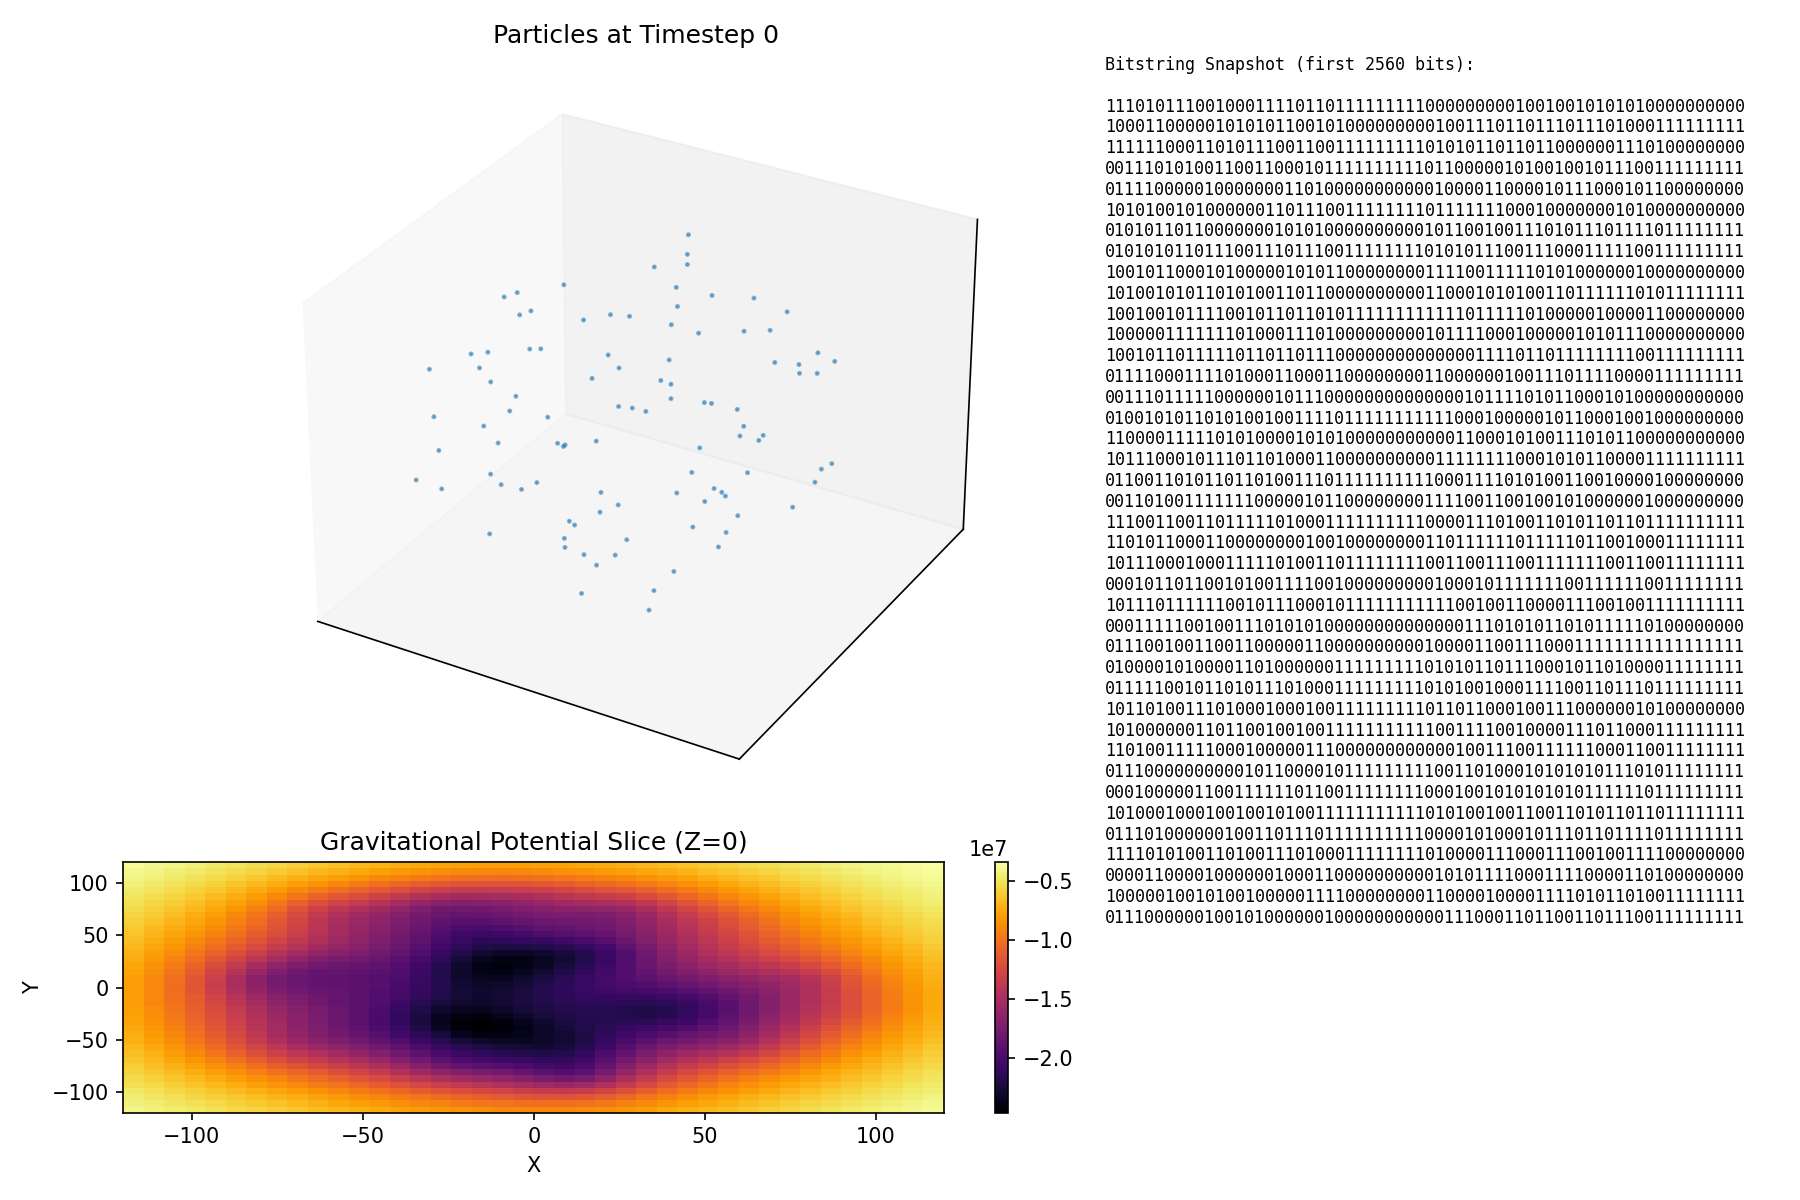
\includegraphics[width=\textwidth]{figures/collapse_0.png}
  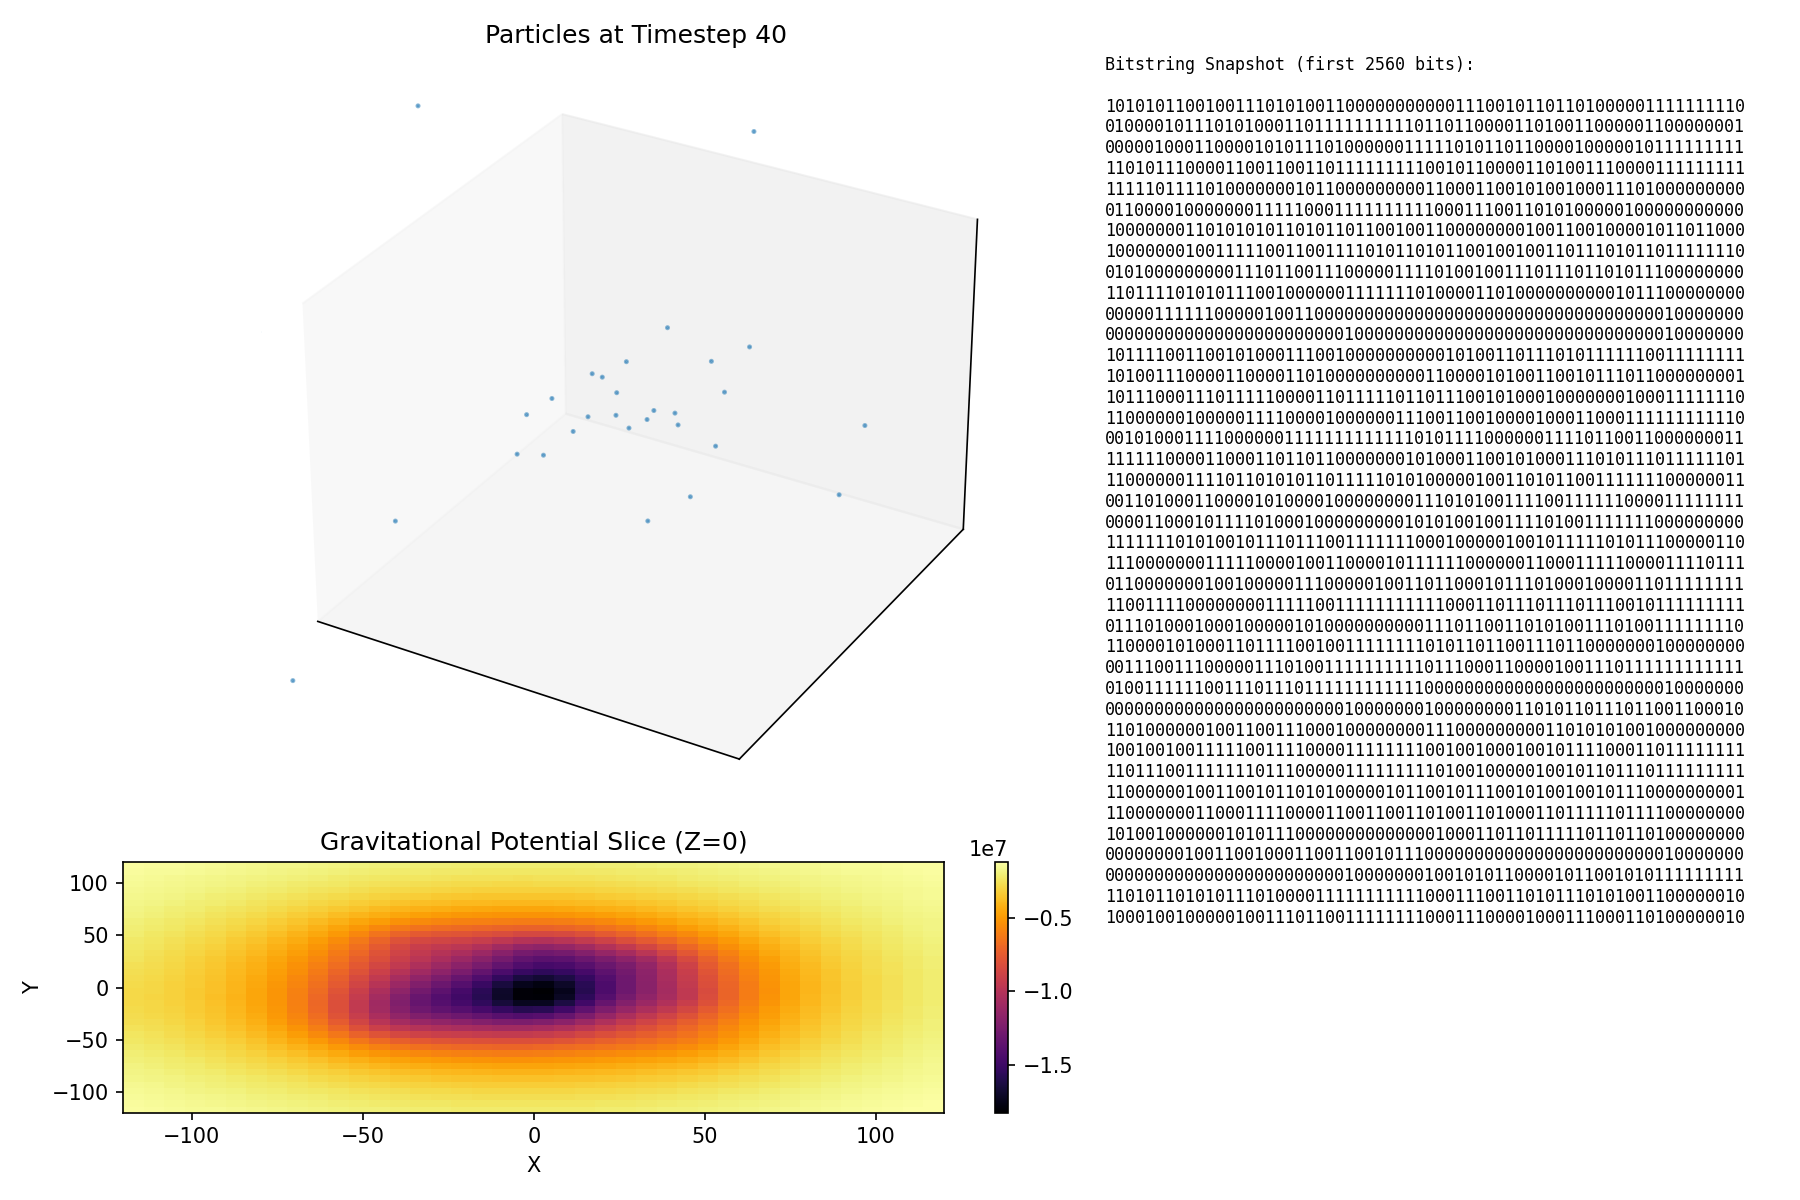
\includegraphics[width=\textwidth]{figures/collapse_40.png}
  \caption{Collapse of geometry. Left: early stage with high entropy and distributed particle positions. Right: late stage with low entropy and spatial convergence.}
  \label{fig:spacetime_collapse}
\end{figure}



\section{Conclusion}


We have formalized and supported the \textbf{Entropy--Singularity Lemma}: that vanishing entropy in an informationally defined system necessarily corresponds to a pointlike geometric collapse.

All tested gravity models, data representations, and coordinate systems demonstrated vanishing entropy near the singularity. This phenomenon is \textit{invariant} under coordinate transformations, data encodings, and gravitational frameworks.

Shannon entropy reliably reflects the underlying geometric collapse, enabling singularities to be analyzed using information-theoretical methods---even though the singularity itself lies outside the domain of the general relativity manifold.

This offers an \textbf{objective, observer-independent informational foundation} for understanding the nature of singularities.


\section{Discussion and Implications}

Our simulations confirm the Entropy--Singularity Lemma in a computational context. While the total thermodynamic entropy of the full black hole system increases (consistent with the second law), the local entropy of spatial encoding decreases near the singularity. This reflects a narrowing of accessible states and growing determinism in geometry.

Importantly, this is not a contradiction of thermodynamics. Instead, it distinguishes between global physical entropy and local representational entropy used in encoding spacetime geometry. Our findings suggest that entropy provides an absolute informational scale, with zero entropy corresponding to the collapse of space.

This perspective allows us to reinterpret gravitational singularities not as breakdowns of physical law, but as informational fixed points: locations in the computational evolution of the universe where no further geometric variability is present.


\section{Future Work}


Future work will extend this framework to entropy increase, simulating early-universe inflation, structure formation, and entropy-driven emergence of geometric complexity. We also intend to connect these results with observer-based models of consciousness and time.

\appendix

\section{Appendix: Bitstring Encoding}

To serialize a geometric state into a bitstring $b \in \{0,1\}^L$:
\begin{enumerate}
  \item Quantize continuous coordinates: $\mathbb{R} \to \mathbb{Z}$
  \item Convert integers to binary strings of fixed width $k$
  \item Concatenate binary segments into a full state bitstring
\end{enumerate}

To compute entropy:
\[
  H(b) = -p_0 \log_2 p_0 - p_1 \log_2 p_1
\]
where $p_0$ and $p_1$ are empirical frequencies of bits in $b$.

\printbibliography

\end{document}
